\documentclass[11pt,a4paper,uplatex,dvipdfmx]{ujarticle} 		% for uplatex
%\documentclass[11pt,a4j,dvipdfmx]{jarticle} 					% for platex
\input{pieces/form00_header} % pieces
\input{pieces/kakenhi7} % pieces
\input{pieces/form01_dcpd_header} % pieces
\input{pieces/hook3} % pieces
%#Name: dc
\input{pieces/form03_dcpd_headers} % pieces
\input{pieces/form04_dc_header} % pieces
% ===== Global definitions for the Kakenhi form ======================
%　基本情報
%
%------ 研究課題名  -------------------------------------------
\newcommand{\研究課題名}{打ち切り超局所台の関手的性質の研究とMorse理論への応用}

%----- 研究機関名と研究代表者の氏名-----------------------
\newcommand{\研究機関名}{北海道大学}
\newcommand{\研究代表者氏名}{大柴寿浩}
\newcommand{\me}{\underline{\underline{T.~Oshiba}}} 
\input{pieces/inst_general_images} % pieces
% user07_header
% ===== my favorite packages ====================================
% ここに、自分の使いたいパッケージを宣言して下さい。
\usepackage{wrapfig}
\usepackage{amsfonts}
\usepackage{amsmath}
\usepackage[psamsfonts]{amssymb}
\usepackage{amsthm}
\usepackage{mathrsfs}
\usepackage{booktabs}

%\usepackage{amssymb}
%\usepackage{mb}
%\DeclareGraphicsRule{.tif}{png}{.png}{`convert #1 `dirname #1`/`basename #1 .tif`.png}
\usepackage{lineno}
\usepackage{color}
\usepackage{xcolor}
\definecolor{darkgreen}{rgb}{0,0.45,0} 
\definecolor{darkred}{rgb}{0.90,0,0}
\definecolor{darkblue}{rgb}{0,0,0.6} 
\usepackage{enumerate}

% ===== my personal definitions ==================================
% ここに、自分のよく使う記号などを定義して下さい。
\newcommand{\klpionn}{K_L \to \pi^0 \nu \overline{\nu}}
\newcommand{\kppipnn}{K^+ \to \pi^+ \nu \overline{\nu}}
\newcommand{\ctext}[1]{\raise0.2ex\hbox{\textcircled{\scriptsize{#1}}}}

\newcommand{\HOM}{\mathop{\mathcal{H}\hspace{-2pt}om}\nolimits}%内部Hom
\newcommand{\RHOM}{\mathop{\mathrm{R}\hspace{-1.5pt}\HOM}\nolimits}

% ----- 業績リスト用 -------------
\newcommand{\paper}[6]{%
	% paper{title}{authors}{journal}{vol}{pages}{year}
	\item ``#1'', #2, #3 {\bf #4}, #5 (#6).			% お好みに合わせて変えてください。
}

\newcommand{\etal}{\textit{et al.\ }}
\newcommand{\ca}[1]{*#1}	% corresponding author;   \ca{\yukawa}  みたいにして使う
\newcommand{\invitedtalk}{招待講演}

\newcommand{\yukawa}{H.~Yukawa}					% no underline
%\newcommand{\yukawa}{\underline{\underline{H.~Yukawa}}}	% with 2 underlines
\newcommand{\tomonaga}{S.~Tomonaga}

\newcommand{\prl}{Phys.\ Rev.\ Lett.\ }		% よく使う雑誌も定義すると楽

% ===== 欄外メモ ==================
\newcommand{\memo}[1]{\marginpar{#1}}
%\renewcommand{\memo}[1]{}	% 全てのメモを表示させないようにするには、行頭の"%"を消す

%\input{../../sample/simple/contents}	% skip
\input{pieces/hook5} % pieces

\begin{document}
\input{pieces/hook7} % pieces
%#Split: 01_background  
%#PieceName: p01_background
\input{pieces/p01_background_00}
\section{研究の概要と位置づけ}
%　　　　＜＜最大　1ページ＞＞

%s03_abst_background
\noindent
\underline{\textbf{研究課題名：\研究課題名}}
%begin 研究科題名及び研究の概要 ＝＝＝＝＝＝＝＝＝＝＝＝＝＝＝＝＝＝＝＝
%研究課題名：打ち切り超局所台を用いた層理論の研究
%\textbf{【研究の概要】}
\vspace{-10pt}
\paragraph{【研究の概要】}
多様体\(M\)上の層の複体\(F\)に対して，
\textcolor{darkred}{\textbf{超局所台}}\(\mathrm{SS}(F)\)という，
余接束\(T^{\ast}M\)の部分集合が定義される．
さらに，それを精密化した\textcolor{darkred}{\textbf{打ち切り超局所台}}\(
	\mathrm{SS}_{k}(F)
\)が各整数\(k\)に対して定義される．
%ここで一般に\(\mathrm{SS}_{k}(F)\subset\mathrm{SS}(F)\)がなりたつ．
この打ち切り超局所台に関して，
以下の2つを目標に研究を行う．
%具体的には，

第1に，打ち切り超局所台を用いて，
\textcolor{darkred}{\textbf{層係数Morse理論を精密化}}する．
%ことを目指す．
\cite{ST92}において，Morse理論は層係数に一般化された．
そこでは，
%普通のMorse理論での，
関数の臨界点にあたる条件が，
超局所台を用いた
%て述べられる
条件に置き換わる．
その条件を打ち切り超局所台を用いたものに取り替えることで，
%得られる結果も精密化できることが期待される．
%その意味で，
層係数Morse理論を精密化するのが目標の一つである．

第2に，\textcolor{darkred}{\textbf{打ち切り超局所台の関手的性質を調べる}}．
打ち切り超局所台の関手的性質として基本的なもの%，
%例えば，順像・逆像・外部テンソル積での振る舞い
は，
\cite{KMS03}で調べられている．
ところが，例えばFourier--Sato変換に
%関する振る舞い
関して
は調べられていないなど，
%打ち切り超局所台の関手的性質については，
明らかになっていない部分も多い．
そのような関手的性質を調べるのがもう一つの目標である．


%超局所層理論の，
%特異点論・シンプレクティック幾何・\(D\)加群論を含む様々な分野への
%応用が盛んになっている．
本研究の完成時には，
%それら
層理論を様々な分野に応用するにあたって，
%ための
\textcolor{darkred}{
	\textbf{適用条件の確認がより簡明になる}
}とともに，
\textcolor{darkred}{
	\textbf{コホモロジーのより詳細な情報が得られる}
}ことが期待される．
%end 研究科題名及び研究の概要 ＝＝＝＝＝＝＝＝＝＝＝＝＝＝＝＝＝＝＝＝＝
\vspace{-10pt}
%begin 研究目的や背景などの概要 ＝＝＝＝＝＝＝＝＝＝＝＝＝＝＝＝＝＝＝＝
%\textbf{【当該分野の状況や課題等の背景】}
\paragraph{【当該分野の状況や課題等の背景】}
超局所台は，層\(F\)を係数とするコホモロジーが，
各点の周りで，
\textcolor{darkred}{\textbf{どの方向に拡張できないかを記述}}する．
その理論は超局所層理論と呼ばれ，
近年，\cite{Nad09,NZ09}や\cite{Tam18}に代表されるように，
シンプレクティック幾何への応用が盛んになってきた．
とりわけ\cite{GKS12}では，層係数Morse理論を効果的に用いて，
シンプレクティック幾何における重要な問題である
Arnoldの分離不能性定理の新しい証明を与えた．
その他にも，\(D\)加群論・特異点論など，様々な分野に応用されている．

他方，柏原--Fernandes--Schapira\cite{KMS03}は，
\(D\)加群の解の伝播の研究を通じて，
打ち切り超局所台を定義した．
打ち切り超局所台は\(F\)係数コホモロジーのうち，\textcolor{darkred}{
	\textbf{固定した次数\(k\)以下のものが拡張できない方向を記述}
}する．
この意味で，打ち切り超局所台は超局所台の
精密化である．
\cite{KMS03}では，打ち切り超局所台に関する
いくつかの性質が成り立つことが示されている．
例えば，層の外部テンソル積に関する超局所台の振る舞いについては，
打ち切り超局所台を用いることで，より細かい情報が得られることが示された．
しかし，関手的性質を始め，
その一般的な性質は調べ尽くされているとは言い難い．
それにも関わらず，2010年代以降に大きな発展は
見られず，\textcolor{darkred}{\textbf{ほとんど手付かず}}の状態にあると言ってよい．

%これに関しては十分に調べられているとは言い難い．
%例えば，超局所Morseの補題は，
%打ち切り超局所台を用いて精密化することができるが，それは論文になっていない．

%end 研究目的や背景などの概要 ＝＝＝＝＝＝＝＝＝＝＝＝＝＝＝＝＝＝＝＝
\vspace{-10pt}
%begin 本研究の着想に至った経緯など ＝＝＝＝＝＝＝＝＝＝＝＝＝＝＝＝＝＝＝＝
%\textbf{【本研究計画の着想に至った背景】}
\paragraph{【本研究計画の着想に至った背景】}
以上で述べた状況の中で，超局所Morseの補題と呼ばれる，
超局所台を用いて定式化される主張が，
打ち切り超局所台を用いるとコホモロジーの次数に関する情報も
含む形に精密化できることに気づいた．
これを援用して，\textcolor{darkred}{
	\textbf{超局所層理論における種々の命題が，
	打ち切り超局所台により改良できる}
}のではないかと思い至った．
また，それを研究する過程でも，
\textcolor{darkred}{\textbf{打ち切り超局所台に関する一般論の構築が必要}}であると考えるに至った．
%end 本研究の着想に至った経緯など ＝＝＝＝＝＝＝＝＝＝＝＝＝＝＝＝＝＝＝＝

%begin 参考文献 ＝＝＝＝＝＝＝＝＝＝＝＝＝＝＝＝＝＝＝＝＝＝＝＝＝＝＝＝＝
%\vspace{11pt}
\begin{thebibliography}{99}
	{\small
	\bibitem[KMS03]{KMS03} M.~Kashiwara, T.~M.~Fernandes, 
	P.~Schapira, 
	\textit{Truncated Microsupprt and Holomorphic Solutions 
	of \(D\)-modules}, 
	Ann. Scient. \'Ec. Norm. Sup., s\'erie 4, tome 36, 
	pp.583--399, 2003.
	\vspace{-6pt}	
	\bibitem[KS90]{KS90} M. Kashiwara, P. Schapira, \emph{Sheaves on manifolds}, Grundl. math. Wiss., vol. 292, Springer, 1990.
	\vspace{-6pt}
	\bibitem[GKS12]{GKS12} S. Guillermou, M. Kashiwara, P. Schapira, \emph{Sheaf quantization of Hamiltonian isotopies and applications to nondisplaceability problems}, Duke Math. J. 161 (2012), 201--245.
	\vspace{-6pt}
	\bibitem[Nad09]{Nad09} D. Nadler, \emph{Microlocal branes are constructible sheaves}, Selecta Math. 15 (2009), 563--619.
	\vspace{-6pt}
	\bibitem[NZ09]{NZ09} D. Nadler, E. Zaslow, \emph{Constructible sheaves and the Fukaya category}, J. Amer. Math. Soc. 22 (2009), 233--286.
	\vspace{-6pt}
	\bibitem[ST92]{ST92} P.~ Schapira, N.~ Tose, 
    \textit{Morse Inequalities for \(\mathbf{R}\)-constructible Sheaves}, 
    Adv. Math. 93, pp.1--8, 1992. 
	\vspace{-10pt}
	\bibitem[Tam18]{Tam18} D. Tamarkin, \emph{Microlocal condition for non-displaceability}, Springer Proc. Math. Stat., vol. 269, Springer, 2018, 99--223.
	\vspace{-6pt}
	}
\end{thebibliography}
%end 参考文献 ＝＝＝＝＝＝＝＝＝＝＝＝＝＝＝＝＝＝＝＝＝＝＝＝＝＝＝＝＝


\input{pieces/p01_background_01}

%#Split: 02_purpose_plan  
%#PieceName: p02_purpose_plan
\input{pieces/p02_purpose_plan_00}
\section{【２】研究計画（２）研究目的・内容等}
%　　　　＜＜最大　2ページ＞＞
%s02_purpose_plan_dcpd
%\JSPSInstructions		% <-- 留意事項。これは消すか、コメントアウトしてください。
\vspace{-30pt}
%begin 研究目的と研究計画shorter ＝＝＝＝＝＝＝＝＝＝＝＝＝＝＝＝＝＝＝＝
\subsection*{\ctext{1} 研究目的・研究方法・研究内容}
%\vspace{-10pt}
\paragraph{【研究目的】}
本研究の目的は，打ち切り超局所台の一般理論の拡充と，
それによる層係数Morse理論の精密化を図ることである．
\vspace{-10pt}
\paragraph{【研究方法・研究内容】}
以下のとおり行う．
%\vspace{-10pt}

\noindent
\textbf{(1) 層係数Morse理論の精密化}：
打ち切り超局所台を用いることで，層係数Morse理論を精密化する．
特に，Morse不等式を層係数に一般化するにあたり，
\cite{ST92}では，一般の層ではなく，実構成可能層と呼ばれる，
特殊な層に制限している．
そこで，本研究でも，実構成可能層に対する理論を構築することを目指す．

\begin{wrapfigure}{r}{8cm}
	\begin{center}
		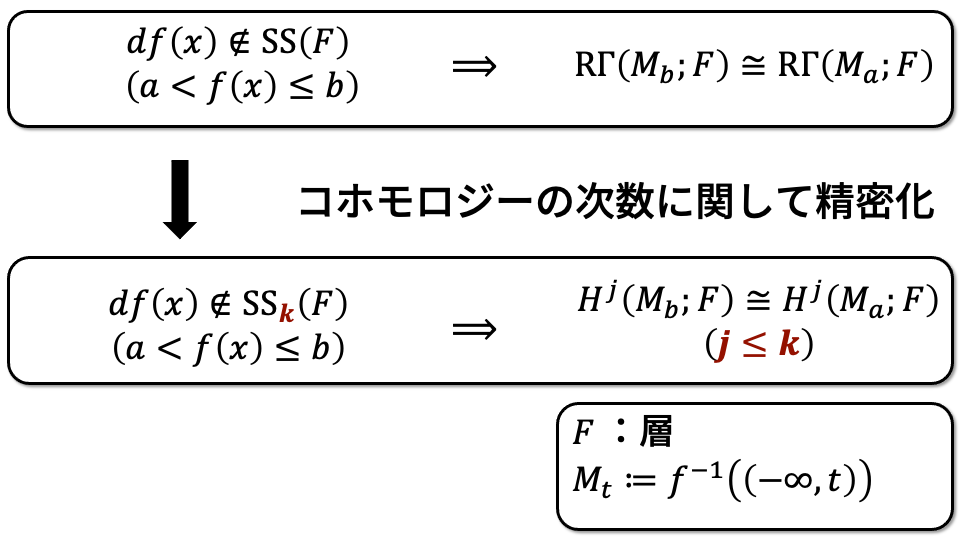
\includegraphics[width=8cm]{figs/dc1-image1.png}
		\caption{研究(1)}
		\label{fig:image1}
	\end{center}
\end{wrapfigure}

\noindent
\textbf{(2) 打ち切り超局所台の関手的性質の探求}：
	%先行研究\cite{KMS03a,KMS03b}での
	%所謂Grothendieckの六則演算のうち，
	%打ち切り超局所台の順像・逆像・テンソル積と，
	%法錐に関する性質が述べられている．
	%ところが，
	%内部Hom関手\(\RHOM\)については
先行研究\cite{KMS03}の手法に基づき，
打ち切り超局所台の関手的性質を調べる．
まず，Fourier--Sato変換の打ち切り超局所台について成り立つ
性質を求める．
さらに，そこから得られる他の関手との関係について調べる．

\noindent
\textbf{(3) 超局所的関手の打ち切り版の構成}\\
\cite{KS90}では，多様体上の層に対し，余接束上の層を対応させる
超局所化関手や，その一般化である\(\mu hom\)関手が定義されている．
これらをコホモロジーの次数に関して分解した，
打ち切り超局所化関手や打ち切り\(\mu hom\)関手を構成し，
その関手的性質を調べる．

%\paragraph*{\ctext{1} 研究目的，研究方法，研究内容}
\subsection*{\ctext{2} どのような計画で，何を，どこまで明らかにしようとするのか}
\paragraph{【年次計画】}
上記(1)--(3) を以下の表\ref{tab1}のとおり行う．

\vspace{-10pt}

\begin{table}[h]
\begin{center}
	\caption{年次計画}
	\label{tab1}
	\begin{tabular}{cc}\toprule
		年度 & 内容 \\\midrule
		2026（1年目）& (1) 層係数Morse理論への応用 \\
		2027（2年目）& (2) Fourier--Sato変換に関する振る舞いの記述\\
		2028（3年目）& (3) 超局所的関手の打ち切り版の構成と性質の調査\\\bottomrule
	\end{tabular}
\end{center}
\end{table}
\vspace{-20pt}
\subparagraph{1年目} 
(1) の層係数Morse理論について，主要な定理であるMorseの不等式を示す．
先行研究\cite{ST92}の設定に基づき，
実構成可能層を考える．関数を一つ固定し，その微分が打ち切り超局所台に
属さないことをコホモロジーの同型に言い換える．
そこから，コホモロジー長完全列を用いて，各次数のコホモロジーの同型を得る．
%\vspace{-10pt}
\subparagraph{2年目}
2年目は，(2) のとおり，打ち切り超局所台の関手的性質について，
Fourier--Sato変換に変換に関する振る舞いと，
%\vspace{-10pt}

\begin{wrapfigure}{r}{8cm}
	\begin{center}
		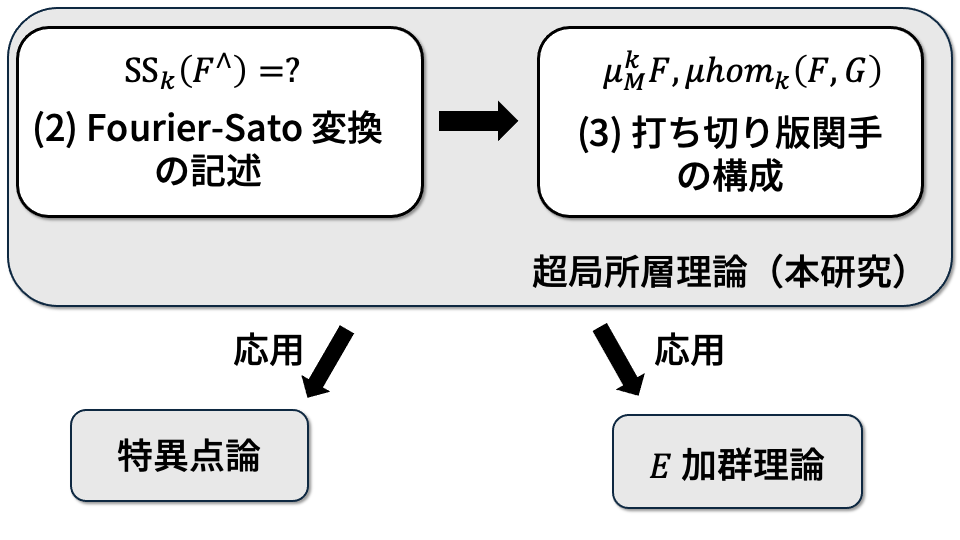
\includegraphics[width=8cm]{figs/dc1-image2.png}
		\caption{研究(2), (3) と他分野との関係}
		\label{fig:image2}
	\end{center}
\end{wrapfigure}

\subparagraph{3年目}
3年目は，超局所化関手と\(\mu hom\)関手の打ち切り版を構成し，その関手的性質を調べる．
2年目の(2) で得られたFourier--Sato変換と
特殊化関手と呼ばれる多様体上の層に対して法束の上の層を対応させる関手の
合成によって，超局所化関手は定義される．

\subsection*{\ctext{3} 研究の特色・独創的な点}

%\vspace{-10pt}

\paragraph{【先行研究との比較】}
古典的なMorse理論では，
与えられた2つの実数\(a<b\)の間にMorse関数\(f\)の
臨界値が存在しなければ，
それぞれの劣位集合は微分同相であることが導かれた．
さらにその帰結として定数層係数のコホモロジーの同型が得られた．
超局所台を用いた層係数Morse理論を扱った先行研究\cite{ST92}では，
\(a<f(x)<b\)のとき，その微分\(df(x)\)が層の超局所台に含まれなければ，
劣位集合上の大域切断関手の導来関手が同型であることが示された．
この先行研究の状況では，余接束の点が超局所台に含まれるかどうかは，
すべてのコホモロジーが同型になるかどうかが判定条件になるので，
各次数のコホモロジーの状況が不明瞭である．
それに対し本研究では，
超局所台を各次数に分解した超局所台を用いるので，
どの次数まで，コホモロジーが同型になるかという，
もっと細かい情報が得られる．

また，先行研究\cite{KMS03a,KMS03b}では，
層の演算に関する打ち切り超局所台の振る舞いを，
順像・逆像・テンソル積については求めている．
さらに，Whitneyの法錐を用いた打ち切り超局所台の記述についても求めている．
しかし，Fourier--Sato変換に関する振る舞いや超局所化関手，
\(\mu hom\)関手との関係については
述べられていない．
これに対し本研究では，
以上の3つの関手と打ち切り超局所台の関係を与える．

\vspace{-10pt}
\paragraph{【本研究の完成時に予想されるインパクト】}
上記(1)--(3)について，対応することを述べる．
(1) が完成した場合，層係数Morse理論の応用が一層容易になる．
特に，
その適用条件が次数のコホモロジーの延長可能性として明示的に記述できるので，
導来圏などの手法に不慣れな研究者でも，
利用することが容易になることが期待される．
%特異点をもつ空間に対するMorse理論への応用が知られているが，

(2), (3) が完成した場合，超局所解析への応用が得られる．
従来の打ち切り超局所台の理論は\(D\)加群論への応用を見込んで展開された．
本研究では，\(D\)加群の超局所化である\(E\)加群にも適用できる．
そのため，\(E\)加群の解の延長可能性について，
コホモロジーの次数に着目した，
より精密な研究が可能となることが期待される．
\vspace{-10pt}
\subsection*{\ctext{4}, \ctext{5}：該当しない}
%\vspace{1cm}
\begin{thebibliography}{99}
		{\small
		\bibitem[KMS03a]{KMS03a} M.~Kashiwara, T.~M.~Fernandes, 
		P.~Schapira, 
		\textit{Truncated Microsupprt and Holomorphic Solutions 
		of \(D\)-modules}, 
		Ann. Scient. \'Ec. Norm. Sup., s\'erie 4, tome 36, 
		pp.583--399, 2003.
		\vspace{-6pt}	
		\bibitem[KMS03b]{KMS03b} M.~Kashiwara, T.~M.~Fernandes, 
		P.~Schapira, 
		\textit{Involutivity of Truncated Microsupprts}, 
		Bull. Soc. math. France, 131 (2), 2003, 
		pp.259--266.
		\vspace{-6pt}	
		\bibitem[KS90]{KS90} M. Kashiwara, P. Schapira, \emph{Sheaves on manifolds}, Grundl. math. Wiss., vol. 292, Springer, 1990.
		\vspace{-6pt}
		\bibitem[ST92]{ST92} P.~ Schapira, N.~ Tose, 
		\textit{Morse Inequalities for \(\mathbf{R}\)-constructible Sheaves}, 
		Adv. Math. 93, pp.1--8, 1992. 
		%\vspace{-10pt}
		}
\end{thebibliography}
	
%end 研究目的と研究計画shorter ＝＝＝＝＝＝＝＝＝＝＝＝＝＝＝＝＝＝＝＝
\input{pieces/p02_purpose_plan_01}

%#Split: 03_rights  
%#PieceName: p03_rights
\input{pieces/p03_rights_00}
\section{人権の保護及び法令等の遵守への対応}
%　　　　＜＜最大　1ページ＞＞

% s09_rights
%begin 人権の保護及び法令等の遵守への対応 ＝＝＝＝＝＝＝＝＝＝＝＝＝＝＝＝＝＝＝＝
	該当しない．

	%象の卵のES細胞の培養、象のクローンの生成などは行わない。

	%\LaTeX の便利な機能については、\texttt{egg\_***.tex} や\texttt{sample\_pdf/egg\_***.pdf}をご覧ください。
%end 人権の保護及び法令等の遵守への対応 ＝＝＝＝＝＝＝＝＝＝＝＝＝＝＝＝＝＝＝＝

\input{pieces/p03_rights_01}

%#Split: 04_abilities  
%#PieceName: p04_abilities
\input{pieces/p04_abilities_00}
\section{【４】研究遂行力の自己分析}
%　　　　＜＜最大　2ページ＞＞

% s14_abilities
%\SelfReviewInstructions\\% <-- 留意事項：これは消すか、コメントアウトしてください。
\noindent
\textbf{(1) 研究に関する自身の強み}\\
%\PapersInstructions\\ %<-- 留意事項：これは消すか、コメントアウトしてください。
%begin 自己分析 ＝＝＝＝＝＝＝＝＝＝＝＝＝＝＝＝＝＝＝＝
\begin{itemize}
	\item 文献調査が得意
	\item プレゼンテーション能力
	\item 新しい理論を積極的に勉強する
\end{itemize}
	\paragraph{分野を問わず広く学ぶ意欲がある}
	申請者は数学に限らず、物理学や語学、言語哲学などの人文系の学問にも
	広く関心を持って自主的に勉強してきた。

	\paragraph{文献調査能力}
	申請者は

	\paragraph{プレゼンテーション能力}
	申請者はプレゼンテーション能力に長けている。

%end 自己分析 ＝＝＝＝＝＝＝＝＝＝＝＝＝＝＝＝＝＝＝＝

\vspace{5mm}
\noindent
\textbf{(2) 今後研究者として更なる発展のため必要と考えている要素}\\
%begin 今後必要な要素 ＝＝＝＝＝＝＝＝＝＝＝＝＝＝＝＝＝＝＝＝
\begin{itemize}
	\item 共同研究者を増やす。
	\item 基礎的な知識を身につける。
\end{itemize}
%end 今後必要な要素 ＝＝＝＝＝＝＝＝＝＝＝＝＝＝＝＝＝＝＝＝

\input{pieces/p04_abilities_01}

%#Split: 99_tail
\input{pieces/hook9} % pieces
\end{document}

